\documentclass{beamer}

\usepackage{txfonts}
\usepackage{hyperref}
\usepackage{fancybox}
\usepackage{xfrac}
\usepackage{cancel}

\newcommand{\heart}{\ensuremath\heartsuit}

\makeatletter
\newcommand{\thnum}[1]{#1\renewcommand{\@currentlabel}{#1}}
\makeatother

\usepackage{mathtools,amssymb}
\newcommand{\myarrow}{\scalebox{2}[2]{$\mathclap{\curvearrowleft}\mkern2.2mu
                                                 \mathclap{\curvearrowright}$}}

\DeclareMathOperator{\Bin}{\mathrm{Bin}}
\DeclareMathOperator{\Max}{\mathrm{Max}}
\DeclareMathOperator{\Cov}{\mathrm{Cov}}
\DeclareMathOperator{\Covr}{\mathrm{Covr}}
\DeclareMathOperator{\Corr}{\mathrm{Corr}}

\hypersetup{colorlinks=false,linkbordercolor=red,linkcolor=green,pdfborderstyle={/S/U/W 1}}

\addtobeamertemplate{navigation symbols}{}{ \hspace{1em}    \usebeamerfont{footline}%
    \insertframenumber / \inserttotalframenumber}

\geometry{papersize={15cm,15cm}}
\usepackage{lipsum}

\makeatletter
\newenvironment<>{contdproof}[1][\proofname]{%
    \par
    \def\insertproofname{#1\@addpunct{.}}%
    \usebeamertemplate{proof begin}#2}
  {\usebeamertemplate{proof end}}
\makeatother


\setbeamertemplate{theorems}[numbered]

\newtheorem{remark}{Remark}



\newtheorem*{nonumdefinition}{Definition}
\newtheorem*{nonumproblem}{Problem}
\newtheorem*{nonumcorollary}{Corollary}
\newtheorem*{nonumlemma}{Lemma}
\newtheorem*{nonumproof}{Proof}
\newtheorem*{nonumtheorem}{Theorem}
\newtheorem*{nonumremark}{Remark}
\newtheorem*{answer}{Answer}
\newtheorem*{nonumremarks}{Remarks}
\newtheorem*{nonumexamples}{Examples}
\newtheorem*{nonumsolution}{Solution}
\newtheorem*{nonumexample}{Example}
\newtheorem*{nonumproposition}{Proposition}
\newtheorem{proposition}[theorem]{Proposition}

\usepackage{tikz}
\newcommand*\mycirc[1]{%
  \tikz[baseline=(C.base)]\node[draw,circle,inner sep=.7pt](C) {#1};\:
}

\newcommand\myheading[1]{%
  \par\bigskip
  {\color{blue}{\large #1}}\par\smallskip}

%\usetheme{Warsaw}
%\usetheme{Berkeley} %sample 1

\usetheme{Berlin} % sample 2
%\usetheme{AnnArbor} % sample 3

\let\otp\titlepage
\renewcommand{\titlepage}{\otp\addtocounter{framenumber}{-1}}

\title{Lecture 18 : Pairs of Continuous Random Variables}
\author{}
\date{}

\begin{document}
\begin{frame}[plain]
\titlepage
\end{frame}

\begin{frame}
\begin{nonumdefinition}
Let $X$ and $Y$ be continuous random variables defined on the same sample space $S$. Then the \underline{joint} probability density function, joint $pdf$, $f_{X,Y}(x,y)$ is the function such that 
\begin{equation*}
P((X,Y)\in A)=\underbrace{\iint\limits_{A} f_{X,Y}(x,y)dx \ dy}_{\text{double integral}}\tag{*}\label{eq-*}
\end{equation*}
for any region $A$ in the plane.
\end{nonumdefinition}
\end{frame}

\begin{frame}
Again the geometric interpretation of \eqref{eq-*} is very important

\smallskip
\centerline{
\includegraphics{figure/fig1.eps}}
\smallskip
\centerline{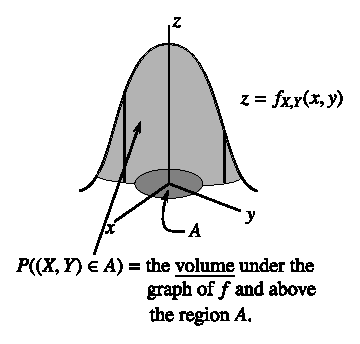
\includegraphics{figure/fig2.eps}}
\end{frame}

\begin{frame}
For $f(x,y)$ to be a joint $pdf$ for some pair of random variables $X$ and $Y$ it is necessary and sufficient that
$$
f(x,y)\geq 0,\quad \text{all}\quad x,y
$$
and
$$
\int\limits^{\infty}_{-\infty}\int\limits^{\infty}_{-\infty}f(x,y)dx \ dy=1
$$
or geometrically, the total volume under the graph of $f$ has to be $1$.
\end{frame}

\begin{frame}
\myheading{Example \thnum{5.3}\label{example5.3} (from text)}

A bank operates a drive-up window and $a$ walkup window. On a randomly selected day, let
\begin{center}
\begin{tabular}{r@{\,}c@{\,}l}
$X$ & = & proportion of time the\\
    &   & drive-up facilty is in use.\\[5pt]
$Y$ & = & proportion of time the\\
    &   & walk-up facilty is in use.
\end{tabular}
\end{center}
The set of possible outcomes for the pair $(X,Y)$ is the square
$$
R=\{(x,y), \ 0\leq x\leq 1, \ 0\leq y\leq 1\}
$$
\centerline{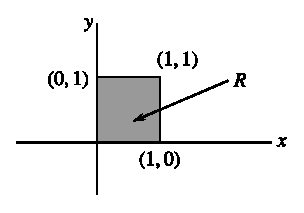
\includegraphics{figure/fig3.eps}}
\end{frame}

\begin{frame}
Suppose the joint $pdf$ of $(X,Y)$ is given by
$$
f_{x,y}(x,y) =
\left\{
\begin{array}{cl}
\sfrac{6}{5}(x+y^{2}), & \begin{array}{@{}l}
                         0\leq x\leq 1\\
                         0\leq y\leq 1
                        \end{array}\\[8pt]
0, & \text{otherwise}
\end{array}
\right.
$$
Find the probability that neither facilty is in use more than $\sfrac{1}{4}$ of the time.

\begin{nonumsolution}
Neither facilty is in use more than $\dfrac{1}{4}$ of the time when re-expressed in terms of $X$ and $Y$ is
$$
X\leq \frac{1}{4} ~ \left(\text{the drive-up facilty is in use $\leq\dfrac{1}{4}$ of the time}\right)
$$
and
$$
Y\leq \frac{1}{4} ~ \left(\text{the walk-up facilty is in use $\leq \dfrac{1}{4}$ of the time}\right)
$$
\end{nonumsolution}
\end{frame}

\begin{frame}
\begin{nonumsolution}[Cont.]
The author formulated the problem in a confusing fashion, don't worry about it.

So we want
$$
P\left(0\leq X\leq \frac{1}{4}, \ 0\leq Y\leq \dfrac{1}{4}\right)
$$
or
$$
P((X,Y)\in S)
$$
where $S$ is the small square

\smallskip
\centerline{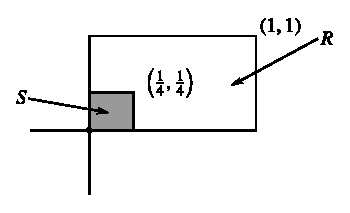
\includegraphics{figure/fig4.eps}}
\smallskip
This probability is given by
\begin{align*}
& \int\limits^{\frac{1}{4}}_{0}\int\limits^{\frac{1}{4}}_{0}\frac{6}{5}(x+y^{2})dx \ dy\\[3pt]
&\quad \iint\limits_{S} \frac{6}{5}(x+y^{2})dx \ dy\tag{$\sharp$}\label{eq-sharp}
\end{align*}
\end{nonumsolution}
\end{frame}

\begin{frame}
\begin{nonumremark}
For general $(X,Y)$ we have
\begin{align*}
& P(a\leq X\leq b, \ c\leq Y\leq d)\\[3pt]
&\quad =\int\limits^{b}_{a}\int\limits^{d}_{c}f_{X,Y}(x,y)dx \ dy
\end{align*}
Let's do the integral \eqref{eq-sharp}. We will do the $x$-integration first. So

\smallskip
\centerline{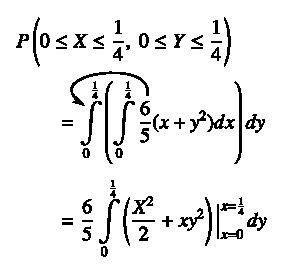
\includegraphics{figure/fig5.eps}}
\end{nonumremark}
\end{frame}

\begin{frame}
\begin{nonumremark}[Cont.]
\begin{align*}
&= \frac{6}{5}\int\limits^{\frac{1}{4}}_{0}\left(\frac{1}{32}+\frac{y}{4}\right)dy\\[3pt]
&= \frac{6}{5}\left[\left(\frac{y}{32}+\dfrac{y^{3}}{12}\right) \Big|^{y=\frac{1}{4}}_{y=0}\right]\\[3pt]
&= \frac{6}{5} \left[\frac{1}{128}+\frac{1}{(64)(12)}\right]\\[3pt]
&= \left(\frac{6}{5}\right)\left(\frac{1}{64}\right)\left(\frac{1}{2}+\frac{1}{12}\right)\\[3pt]
&= \left(\frac{\cancel{6}}{5}\right)\left(\frac{1}{64}\right)\left(\frac{7}{\begin{array}{c}\cancel{12}\\ 2\end{array}}\right)\\[3pt]
&= \frac{7}{640}
\end{align*}
An exercise in the forgotten art of fractions- more of the same later.
\end{nonumremark}
\end{frame}

\begin{frame}
\myheading{More Theory Marginal Distributions in the Continuous Case}

\begin{nonumproblem}
Suppose you know the joint $pdf$ $f_{X,Y}(x,y)$ of $(X,Y)$. How do you find the individual $pdf$'s $f_{X}(x)$ of $X$ and $f_{Y}(y)$. The answer is 
\end{nonumproblem}

\begin{nonumproposition}
\begin{equation*}
\begin{aligned}
\text{\rm(i)}~~ & f_{X}(x) = \int\limits^{\infty}_{-\infty} f_{X,Y}(x,y)dy\\
\text{\rm(ii)}~~ & f_{Y}(y)=\int\limits^{\infty}_{-\infty}f_{X,Y}(x,y)dx
\end{aligned}\tag{*}\label{addeq-*}
\end{equation*}
\end{nonumproposition}
\end{frame}

\begin{frame}
\begin{nonumproposition}[Cont.]
The formula \eqref{addeq-*} is the continuous analogue of the formula for the discrete case. Namely
\end{nonumproposition}

\underline{Discrete Case}
$$
f_{X}(x)=\sum\limits_{\text{all}_{y}}f_{X,Y}(y)
$$
\underline{Continuous Case}
$$
f_{X}(x)=\int\limits^{\infty}_{-\infty}f_{X,Y}(x,y)dy
$$
In the first case we sum away the ``extra variable'' $y$ and in the second case we integrate it away.

By analogy once again we call $f_{X}(x)$ and $f_{Y}(y)$ (obtained via \eqref{addeq-*}) the marginal densities or marginal $pdf$'s.
\end{frame}

\begin{frame}
Note the $f_{X}(x)$ and $f_{Y}(y)$ are the two partial definite integrals of $f_{X,Y}(x,y)$ - see Lecture 16.

\myheading{Example \thnum{5.4}\label{example5.4}}

We compute the two marginal $pdf$'s for the bank problem, Example \ref{example5.3}.

\smallskip
\centerline{
\includegraphics{figure/fig6.eps}}
\smallskip

The formula for $f_{X}(x)$ says you integrate $f_{X,Y}(x,y)$ over the vertical
\end{frame}

\begin{frame}
line passing through $x$.

If $x$ does not satisfy $0\leq x\leq 1$ then the vertical line does not pass through the square $R$ where $f_{X,Y}(x,y)$ is non zero

\smallskip
\centerline{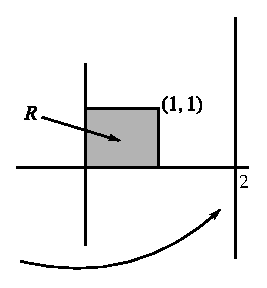
\includegraphics{figure/fig7.eps}}
\smallskip

You get $f_{X}(2)$ by integrating over the line $x=2$ above which $f_{X,Y}(x,y)=0$.

Equivalently (without geometry)
$$
f_{X}(2)=\int\limits^{\infty}_{-\infty}f_{X,Y}(2,g)dy=\int\limits^{\infty}_{-\infty}0 \ dy =0
$$
\end{frame}

\begin{frame}
Now we finish the job
\begin{align*}
& \int\limits^{1}_{0}\frac{6}{5}(x+y^{2})dy=\frac{6}{5}\int\limits^{1}_{0}(x+y^{2})dy\\[3pt]
&\quad =\frac{6}{5}\left(xy+\frac{y^{3}}{3}\right)\Big|^{y=1}_{y=0}=\frac{6}{5}\left(x+\frac{1}{3}\right)
\end{align*}
Similarly
\begin{align*}
f_{Y}(y) &=
\left\{
\begin{array}{cl}
\frac{6}{5}\int\limits^{1}_{0}\frac{6}{5}(x+y^{2})dx, & 0\leq y\leq 1\\[3pt]
0, & \text{otherwise}
\end{array}
\right.\\
&= \left\{
\begin{array}{cl}
\frac{6}{5}y^{2}+\frac{3}{5}, & 0\leq y\leq 1\\
0, & \text{otherwise}
\end{array}
\right.
\end{align*}
\end{frame}

\begin{frame}
\myheading{Independence of Two Continuous Random Variables}

\begin{nonumdefinition}
Two continuous random variables $X$ and $Y$ are independent of their joint $pdf$ $f_{X,Y}(x,y)$ is the product of the two marginal $pdf$'s $f_{X}(x)$ and $f_{Y}(y)$ so
$$
f_{X,Y}(x,y)=f_{X}(x)f_{Y}(y)
$$
This not true for the bank example pg. 5.

\smallskip
\centerline{
\includegraphics{figure/fig8.eps}}
\end{nonumdefinition}
\end{frame}

\begin{frame}
\myheading{Covariance and Correlation of Pairs of Continuous Random Variables}

We continue with a pair of continuous random variables $X$ and $Y$ as before. Again we define
$$
\Cov (X,Y)=E(XY)-E(X)E(Y)
$$
and
$$
\rho_{x,Y}=\Corr (X,Y)=\dfrac{\Cov (X,Y)}{\sigma_{X}\sigma_{Y}}
$$
But now
$$
E(XY)=\int\limits^{\infty}_{-\infty}\int\limits^{\infty}_{-\infty}xy \ f_{X,Y}(x,y)dx \ dy
$$
\end{frame}

\begin{frame}
We will now compute the $\Cov(X,Y)$ and $\Corr(X,Y)$ for the bank problem. So
\begin{align*}
f_{X,Y}(x,y) &=
\left\{
\begin{array}{cl}
\frac{6}{5}(x+y^{2}), & 
\begin{array}{l}
0\leq x\leq 1\\
0\leq y\leq 1
\end{array}\\
0, & \text{otherwise}
\end{array}
\right.\\
f_{X}(x) &= \left\{
\begin{array}{cl}
\frac{6}{5}\left(x+\frac{1}{3}\right), & 0\leq x\leq 1\\
0, & \text{otherwise}
\end{array}
\right.\\
f_{Y}(y) &= \left\{
\begin{array}{cl}
\frac{6}{5}y^{2}+\frac{3}{5}, & 0\leq y\leq 1\\
0, & \text{otherwise}
\end{array}
\right.
\end{align*}
Let's first do the calculations for $X$ and $Y$ - we need
$$
E(X), E(Y),\sigma_{X}=\sqrt{V(X)}\text{~~ and~~ } \sigma_{Y}=\sqrt{V(Y)}
$$
\end{frame}

\begin{frame}
\begin{align*}
E(X) &= \int\limits^{1}_{0} x \frac{6}{5}\left(x+\frac{1}{3}\right)dx\\[3pt]
&= \frac{6}{5}\int\limits^{1}_{0}\left(x^{2}+\frac{x}{3}\right)dx=\frac{6}{5}\left(\frac{x^{3}}{3}+\frac{x^{2}}{6}\right)\Big|^{x=1}_{x=0}\\[3pt]
&= \frac{6}{5}\left(\frac{1}{3}+\frac{1}{6}\right)=\frac{6}{5}\left(\frac{3}{6}\right)=\frac{3}{5}\\[3pt]
E(X^{2}) &= \int\limits^{1}_{0}x^{2}\frac{6}{5}\left(x+\frac{1}{3}\right)dx\\[3pt]
&= \frac{6}{5}\int\limits^{1}_{0}\left(x^{3}+\frac{x^{2}}{3}\right)dx=\frac{6}{5}\left(\frac{x^{4}}{4}+\frac{x^{3}}{9}\right)\Big|^{x=1}_{x=0}\\[3pt]
&= \frac{6}{5}\left(\frac{1}{4}+\frac{1}{9}\right)=\frac{6}{5}\left(\frac{13}{36}\right)=\frac{13}{30}\\[3pt]
V(X) &= \frac{13}{30}-\left(\frac{3}{5}\right)^{2}=\frac{13}{30}-\frac{9}{25}=\frac{65-54}{150}=\frac{11}{150}\\[3pt]
\sigma_{X} &= \sqrt{\frac{11}{150}}=\frac{1}{5}\sqrt{\frac{11}{6}}
\end{align*}
\end{frame}

\begin{frame}
\begin{align*}
E(Y) &= \int\limits^{1}_{y}\left(\frac{6}{5}y^{2}+\frac{3}{5}\right)dy\\[3pt]
&= \frac{6}{5}\int\limits^{1}_{0}y^{3}dy+\frac{3}{5}\int\limits^{1}_{0}ydy\\[3pt]
&= \left(\frac{6}{5}\right)\left(\frac{1}{4}\right)+\left(\frac{3}{5}\right)\left(\frac{1}{2}\right)=\frac{6}{20}+\frac{3}{10}=\frac{12}{20}\\[3pt]
E(Y^{2}) &= \int\limits^{1}_{0}y^{2}\left(\frac{6}{5}y^{2}+\frac{3}{5}\right)dy\\[3pt]
&= \frac{6}{5}\int\limits^{1}_{0}y^{4}dy+\frac{3}{5}\int\limits^{1}_{0}y^{2}dy\\[3pt]
&= \left(\frac{6}{5}\right)\left(\frac{1}{5}\right)+\left(\frac{\cancel{3}}{5}\right)\left(\frac{1}{\cancel{3}}\right)=\frac{6}{25}+\frac{??}{5}=\frac{11}{25}\\[3pt]
V(Y) &= \frac{11}{25}-\frac{144}{400}=\frac{176}{400}-\frac{144}{400}=\frac{32}{400}=\frac{2}{25}\\[3pt]
\sigma_{Y} &= \sqrt{\frac{2}{25}}=\frac{1}{5}\sqrt{2}
\end{align*}
\end{frame}

\begin{frame}
Finally we need
\begin{align*}
E(XY) &= \int\limits^{1}_{0}\int\limits^{1}_{0}(xy)\frac{6}{5}(x+y^{2})dx \ dy\\[3pt]
&= \int\limits^{1}_{0}\int\limits^{1}_{0}\underbrace{xy\frac{6}{5}x}_{\text{product function}} \ dx \ dy +\int\limits^{1}_{0}\int\limits^{1}_{0}\underbrace{xy \frac{6}{5}y^{2}}_{\text{product function}}dx \ dy\\[3pt]
&= \frac{6}{5}\left(\int\limits^{1}_{0}x^{2}dx\right)\left(\int\limits^{1}_{0} y \ dy\right)+\frac{6}{5}\left(\int\limits^{1}_{0}x \ dx\right)\left(\int\limits^{1}_{0} y^{3} dy\right)\\[3pt]
&= \left(\frac{6}{5}\right)\left(\frac{1}{3}\right)\left(\frac{1}{2}\right)+\left(\frac{6}{5}\right)\left(\frac{1}{2}\right)\left(\frac{1}{4}\right)\\[3pt]
&= \left(\frac{6}{5}\right)\left(\frac{1}{2}\right)\left(\frac{1}{3}+\frac{1}{4}\right)=\left(\frac{\cancel{6}}{5}\right)\left(\frac{1}{2}\right)\left(\frac{7}{\begin{array}{c}\cancel{12}\\ 2\end{array}}\right)=\frac{7}{20}
\end{align*}
\end{frame}

\begin{frame}
Now we can mop the fruits of our labours.

%\begin{align*}
%\Cov (X,Y) &= E(XY)-E(X)E(Y)\\[3pt]
%           &= \frac{7}{20}-\left(\frac{3}{5}\right)\left(\frac{12}{20}\right)\\[3pt]
%           &= \frac{7}{20}-\frac{36}{100}=\frac{35}{100}-\frac{36}{100}\\[3pt]
%\Cov(X,Y) &= \frac{-1}{100}\\[3pt]
%\Cov(X,Y) &= \frac{\Cov(X,Y)}{\sigma_{X}\sigma_{Y}}=\frac{\frac{-1}{100}}{\left(\frac{1}{5}\sqrt{\frac{11}{6}}\right)\left(\frac{1}{5}\sqrt{2}\right)}\\[3pt]
%          &= \left(\frac{-1}{\cancel{100}}\right)\left(\frac{\cancel{5}}{\sqrt{\frac{11}{\cancel{6}}}}\right)\left(\frac{\cancel{5}}{\sqrt{\cancel{2}}}\right)=-\frac{1}{4}\left(\frac{1}{\sqrt{\frac{11}{3}}}\right)=-\frac{\sqrt{3}}{4\sqrt{11}}
%\end{align*}
\smallskip

\centerline{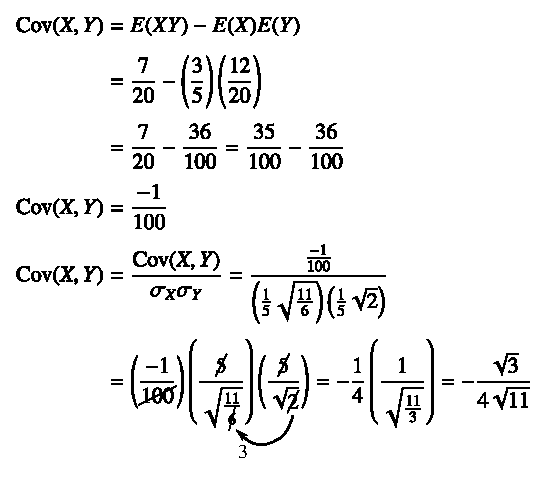
\includegraphics{figure/fig9.eps}}
\end{frame}

\begin{frame}
\myheading{Independence of Continuous Random Variables}

\begin{nonumdefinition}
Two continuous random variables $X$ and $Y$ are independent if the joint $pdf$ is the product of the two marginal $pdf$'s 
$$
f_{X,Y}(x,y)=f_{X}(x)f_{Y}(g)
$$
(so $\Longleftrightarrow$ the joint $pdf$ is a product function)

So in Example \ref{example5.3}, page 4, $X$ and $Y$ are NOT independent.
\end{nonumdefinition}
\end{frame}

\end{document}


